\chapter{Description du travail proposé}
\setlength{\parskip}{2.5ex plus .4ex minus .4ex}

\section{Expression des besoins}
\subsection{Besoins généraux}
Actuellement, le logiciel VLE permet de créer des individus un à un, de leur associer une dynamique, de les relier entre eux et de lancer des simulations. La dynamique de plusieurs individus peut être la même, et peut varier selon les conditions expérimentales qui décrivent les valeurs des paramètres si l'utilisateur les édite.\\
Cependant, il est nécessaire que l'utilisateur édite chaque individu un à un. Comment faire pour modéliser des troupeaux entiers sans avoir ce travail répétitif ~?\\
Pour l'instant, le logiciel VLE propose une interface pour créer la structure du système désirée par l'utilisateur. Puis, il doit programmer en C++ les classes qui définiront les dynamiques des modèles du système lui-même ou bien utiliser un plugin de modélisation comme Forrester par exemple.\\
Si l'utilisateur souhaite modéliser un troupeau, il faudra qu'il crée chaque individu un à un. C'est pourquoi, il était nécessaire de créer une extension du logiciel pour ces cas là. Une extension qui permettrait la création, suppression et la définition d'évènements sur les individus de manière simple et instinctive pour l'utilisateur.\\
L'utilisateur n'aurait donc plus besoin de programmer en C++ ni d'éditer des graphes et réutiliserait le plugin Forrester pour définir les classes d'individus qui serviront de base pour créer chaque individu lors de la simulation.

\subsection{Cas d'utilisations}
Un TP et un modèle type m'ont été donnés afin de me donner une idée des fonctionnalités attendues et de diriger la conception et le développement de mon plugin. Ces exemples ont été réalisés avec le logiciel Modelmaker.\\
Modelmaker est un logiciel de simulation de systèmes dynamiques, dont l'édition des modèles se fait par l'intermédiaire d'un diagramme de Forrester. Les modèles implémentables sont des systèmes d'équations différentielles.\\
Une des fonctionnalités qui nous a particulièrement intéressée dans le cadre du stage est la vectorisation des modèles pour partie ou en totalité qui permet en quelque-sorte d'émuler une approche de modélisation individu centré. D'autre-part, Modelmaker permet aussi de définir des événements qui, en fonction de l'état global du modèle, changent de façon discrète les valeurs des variables d'états. Il me fallait alors adapter les fonctionnalités proposées par Modelmaker afin que ce TP et modèle type soient réalisables avec VLE.\\
\\
Le TP avait pour but de créer 5 modèles dont chacun d'eux possédait un compartiment, le premier se vidant dans le deuxième et si le deuxième atteingnait une certaine valeur, se vidait immédiatement dans un troisième compartiment. Chaque modèle ayant des paramètres de vidange différents.\\
D'autres part, il devait être possible d'offrir à l'utilisateur la possibilité d'observer une ou plusieurs valeurs en particulier. Dans ce cas précis, la somme de tous les compartiments qui se vident.\\
\\
Le modèle type était plus complexe. Il s'agissait de faire naître 10 cellules à t=10, faire croître leurs poids suivant des paramètres distints puis à t=30, repérer la plus grosse cellule et faire décroître les 9 autres.\\ Lorsque la cellule la plus grosse atteint 0.99, 10 autres naissances sont lancées. Si une cellule a un poids inférieur à 0.01, la tuer.
 
\section[IBM] {IBM\footnote{Individual Based Model}}
\subsection{Paradigme IBM}
L'objectif est de pouvoir modéliser en spécifiant au sein d'un système dynamique des populations d'individus.\\
Un individu est formalisé par un système d'équations différentielles et tous les individus d'une population se réfèrent au même système d'équations différentielles.\\
Au sein d'une population les individus peuvent différer de par la valeur de leurs paramètres mais ce n'est pas une obligation.\\
\\
La dynamique des populations est définie par un ensemble d’événements portant sur les individus. Un évènement est défini par des conditions d'activation et des effets.\\
Les conditions d'activation sont exprimées en fonction du temps de la simulation ou de l'état du système simulé. L'état du système est l'union de tous les états des individus.\\
Il existe 3 types d'effet: Création d'un individu, suppression d'un individu et réinitialisation d'un individu.

\subsection{Structure du modèle DEVS}
Chaque individu est un système d'équations différentielles défini par une classe C++. Cette classe est appelée classe d'individu. C'est elle qui doit être défini par l'utilisateur puis qui servira de base pour créer tous les individus de ce type là. C'est pourquoi chaque individu de même type, a la même dynamique, seuls les paramètres peuvent varier entre eux si l'utilisateur souhaite en modifier un ou plusieurs.\\
Chaque individu est indépendant, ils n'intéragissent pas directement les un avec les autres. Ils doivent communiquer par l'intermédiaire d'un même controleur auquels ils sont tous connectés.\\
Chaque port de sortie de chaque individu est relié aux ports d'entrée du controleur, ce qui permet à ce dernier de recevoir des évènements, les traiter et envoyer des réponses adéquates par l'intermédiaire de ses ports de sortie reliés à chaque individu par des ports d'entrée.\\
Lors de la simulation, la dynamique du controleur se met en marche. Elle initialise tous les individus, exécute sa dynamique interne, reçoit les évènements externes et envoie des réponses aux individus. Durant la simulation, le controleur peut à tout moment, créer un nouvel individu, en supprimer ou en modifier les paramètres grâces aux évènements qu'il reçoit en entrée et qu'il peut envoyer en sortie.\\
Par exemple :\\
\noindent\begin{minipage}{\linewidth}% to keep image and caption on one page
\makebox[\linewidth]{%        to center the image
  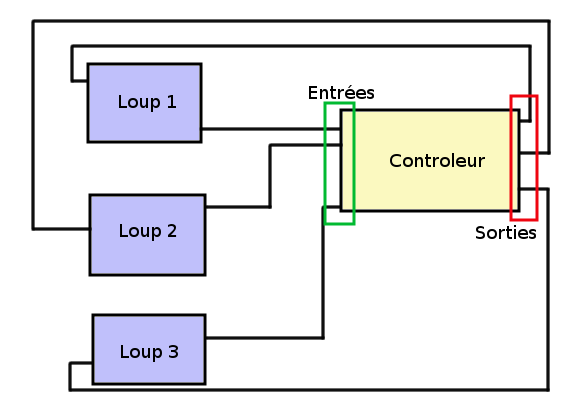
\includegraphics [width=150mm]{images/exemple_ibm.png}}
\captionof{figure}{Trois Loups créés par le controleur lors de la simulation}%\label{visina8}%      only if needed  
\end{minipage}

Le controleur crée les individus ``Loup 1'', ``Loup 2'' et ``Loup 3'' qui sont bien indépendants les uns des autres et tous reliés au controleur comme expliqué au paragraphe précédent. \\

\subsection{IBM dans VLE}
Dans VLE, chaque système ou simulation est représenté par un Vpz qui est un fichier xml où est décrit tout le système. Modèles présents (individus), conditions expérimentales (valeurs des paramètres), classes d'individus, ports d'entrées et de sorties...\\
Dans le Vpz, un controleur est obligatoirement présent s'il s'agit d'un système IBM. Il se crée automatiquement lors de la première ouverture du plugin IBM. \\Ensuite, les modèles souhaités par l'utilisateur sont créés lors de la simulation par le controleur grâce aux classes d'individu définies dans le vpz.\\
Par exemple : \\
\noindent\begin{minipage}{\linewidth}% to keep image and caption on one page
\makebox[\linewidth]{%        to center the image
  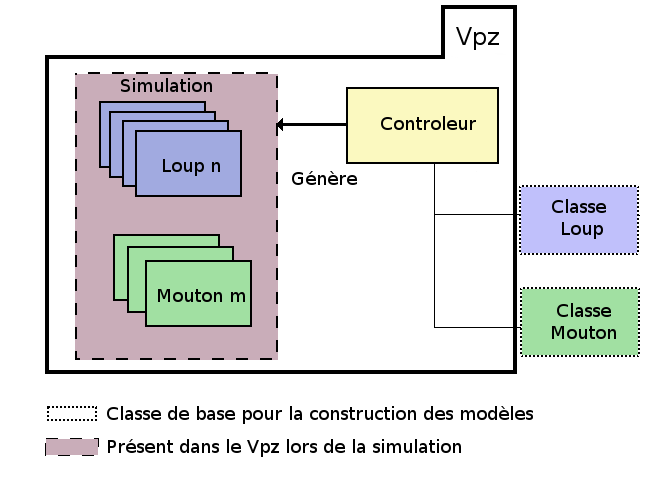
\includegraphics [width=160mm]{images/vpz1.png}}
\captionof{figure}{Composition d'un Vpz}%\label{visina8}%      only if needed  
\end{minipage}

Ici, le controleur crée n Loups et m Moutons lors de la simulation, mais seul le modèle ``Controleur'' est présent dans le vpz. Le controleur est cependant lié aux classes ``Loup'' et ``Mouton'' afin de pouvoir créer les individus.

\section{Fonctionnalités du plugin}
À son ouverture, le plugin récupère toutes les classes d'individu déjà présentes dans le Vpz. Il offre ensuite la possibilité d'ouvrir le plugin Forrester afin de créer d'autres classes et modifier ou supprimer les classes existantes.\\
Afin de manipuler les individus lors de la simulation, le plugin propose un champs de texte afin que l'utilisateur exprime ces besoins par l'intermédiare d'un petit langage simple appelé Lua et quelques extensions que j'aurai développées.\\
Ces besoins peuvent être multiple, ils peuvent avoir un effet sur les individus, création, suppression, modification ou bien renvoyer des informations, valeur d'une variable, nombre d'individus, identifiant d'un individu...\\
D'autre part, le plugin crée automatiquement un exécutive appelé ``Controleur'' à son ouverture. Controleur qui sera chargé de manipuler les individus selon le script qu'aura écrit l'utilisateur, et la dynamique DEVS.\\